%% q-ids --- Computers & Security submission (preprint build).
%% Elsevier elsarticle template. Build: pdflatex -> bibtex -> pdflatex x2.
%% Figures live in figures/ (vector PDF). Bibliography in references.bib.
%%
%% STATUS: Methodology (Sec 3), Results (Sec 4), and Related Work (Sec 2) are drafted.
%% Introduction (Sec 1), Discussion (Sec 5), Conclusion (Sec 6), and the Abstract are
%% STUBS to be written with the co-author -- marked \todo below.

\documentclass[preprint,12pt]{elsarticle}

\usepackage{graphicx}
\usepackage{booktabs}
\usepackage{amsmath,amssymb}
\usepackage{url}
\usepackage[hidelinks]{hyperref}
\graphicspath{{figures/}}

% Lightweight TODO marker (no extra package needed for the preprint build).
\newcommand{\todo}[1]{\textbf{[TODO: #1]}}

\journal{Computers \& Security}

\begin{document}

\begin{frontmatter}

\title{Problem-Space Adversarial Robustness of Classical and Quantum
Machine-Learning Intrusion Detectors: A C2-Beacon Evasion Study}

%% \todo{confirm final title with co-author}

\author[inst1]{Abhishek Ravicharan}
\ead{abhishekravicharan@gmail.com}

\author[inst1]{\todo{Co-author name}}

\affiliation[inst1]{organization={\todo{institution}},
            country={}}

\begin{abstract}
\todo{Write last, with the co-author.} Provisional one-paragraph stub:
We study the robustness of flow-level machine-learning network intrusion detectors to
\emph{realizable} (problem-space) adversarial evasion, using command-and-control (C2) beaconing as an
attack whose detectable signal---timing and size regularity---is exactly a set of parameters the
attacker controls for free. Driving a model-in-the-loop evasion that generates real traffic in an
emulated network and admits only functionality-preserving perturbations, we find that both a classical
neural network and a quantum-classical variational classifier are evaded for 100\% of beacon instances
at a trivial level of timing jitter; that the quantum model offers \emph{no} robustness advantage once
the detection task is made realistic; and that single-axis adversarial training relocates the
vulnerability to a second, equally-free axis rather than closing it.
\end{abstract}

\begin{keyword}
network intrusion detection \sep adversarial machine learning \sep problem-space attacks \sep
command-and-control beaconing \sep quantum machine learning \sep adversarial robustness
\end{keyword}

\end{frontmatter}

% =====================================================================
\section{Introduction}
\label{sec:intro}

\todo{Draft with co-author. Hold until framing (how hard to lead with the quantum angle vs.\ the
problem-space angle) is settled.} Planned contributions:
\begin{itemize}
  \item A model-in-the-loop, functionality-preserving problem-space evasion for flow-level NIDS,
        realized as actual traffic rather than feature-vector perturbation.
  \item The first problem-space robustness comparison of a quantum vs.\ classical detector on a
        security task, finding no quantum advantage.
  \item A concrete demonstration that single-axis adversarial training relocates rather than closes
        the vulnerability (timing~$\rightarrow$~size axis escalation).
\end{itemize}

% =====================================================================
\section{Related Work}
\label{sec:related}

Our work sits at the intersection of four strands: problem-space (realizable) adversarial machine
learning, adversarial evasion against network intrusion detection (NIDS), machine-learning detection
of C2 beaconing, and quantum machine learning for security together with its (separately studied)
adversarial robustness.

\subsection{Problem-space vs.\ feature-space adversarial attacks}
Most adversarial-ML results perturb the \emph{feature vector} directly and measure success in feature
space. Pierazzi et al.~\cite{pierazzi2020} formalized the alternative \emph{problem-space} setting, in
which the attacker must produce a real object (there, an Android app) and the perturbation is
constrained by what is physically realizable---available transformations, preserved semantics, absent
artifacts, and plausibility---because in most domains there is no clean inverse map from a desired
feature vector back to a valid object. Chernikova and Oprea's FENCE~\cite{fence2022} pushed in the
same direction for deep models in \emph{constrained} domains, generating evasions that respect feature
inter-dependencies, with network security among the case studies. These works establish the discipline
we adopt---realizability and functionality preservation as first-class constraints---but for malware
and engineered-feature settings. We carry it into \emph{network flow} NIDS with an in-the-loop traffic
generator: every candidate perturbation is realized as actual packets and admitted only if a functional
oracle confirms the attack still works (Section~\ref{sec:evasion}).

\subsection{Adversarial evasion against NIDS}
Adversarial attacks on ML-based NIDS are by now a large
literature~\cite{nids_survey2023,ennaji2024,nids_understanding2026}. A recurring critique is that many
reported successes are demonstrated in
feature space or under idealized threat models an attacker could not realize on the wire. Apruzzese et
al.~\cite{apruzzese2022} argued for realistic threat models with limited attacker knowledge and
control, and elShehaby and Matrawy~\cite{elshehaby2023} went further, contending that evasion attacks
\emph{remain largely impractical} against real ML-NIDS, especially dynamic ones. A 2024 line of work
begins to close this gap with explicitly problem-space NIDS attacks~\cite{catillo2024}, and related
efforts restrict perturbations to attacker-controllable fields: the controllability-aware framework
of~\cite{li2026} partitions flow features into directly-, indirectly-, and un-controllable groups and
perturbs only the controllable ones, while payload-padding attacks~\cite{jing2025} evade classifiers by
adding bytes that do not disturb transmission.

Our work is a direct response to the realism critique, and sharpens rather than contradicts it. We do
not claim a generic realizable evasion; we isolate one attack class---C2 beaconing---where the
detectable signal (timing/size regularity) is \emph{exactly} a set of parameters the attacker already
controls for free, and show that there the evasion is not only practical but succeeds for 100\% of
instances while a functional oracle confirms the beacon keeps working. The controllable-field idea
of~\cite{li2026} appears here as the physical timing-jitter and size-jitter axes; unlike
feature-masking frameworks, our controllability is grounded in a generator that must emit valid
traffic. This also lets us measure quantities a feature-space attack cannot define honestly: minimal
\emph{realizable} evading perturbation, queries-to-evasion against a black-box verdict, and functional
admissibility.

\subsection{Detecting C2 beaconing}
Flow-level detection of command-and-control beaconing keys on \emph{timing regularity}: a beacon checks
in at a near-constant interval, and the standard statistical signal is a low coefficient of variation
(CV) of inter-arrival times, often combined with anomaly detectors~\cite{yilmaz2026}, with surveys of
C2 technique and defence going back a decade~\cite{gardiner2014}. This is the detection premise we
adopt (our \texttt{cv\_iat} feature is precisely this CV; Section~\ref{sec:features})---and precisely
the premise we attack. The beaconing-detection literature treats timing regularity as a reliable
discriminator; we show that because regularity is an attacker-set parameter with functional slack, a
detector that relies on it is defeated by a cost-free increase in jitter, and that the near-identical
\emph{rigid benign} traffic (NTP, health checks, keepalives) bounds how aggressively any such detector
can tighten without false alarms.

\subsection{Quantum machine learning for intrusion detection}
A growing body of work applies quantum and quantum-classical models---variational quantum classifiers
(VQCs), quantum SVMs, quantum CNNs---to intrusion detection, generally reporting accuracy competitive
with or exceeding classical baselines~\cite{abreu2024,thomos2026,qvcnn2024}, within a broader
QML-for-security literature~\cite{qml_sec_taxonomy2025}. This literature is almost entirely about
\emph{clean} accuracy; it does not evaluate robustness to realizable evasion, and typically works from
static feature datasets. We add the missing axis: a VQC and a classical MLP trained on \emph{matched
inputs} (Section~\ref{sec:detectors}) and compared not on clean accuracy alone but on problem-space
robustness to the same realized attack traffic.

\subsection{Adversarial robustness of quantum classifiers}
Separately from the IDS setting, a quantum-ML-theory literature asks whether quantum classifiers are
\emph{inherently} more robust. Early results showed VQCs are, like classical networks, vulnerable to
adversarial examples~\cite{lu2020,liao2021}, but subsequent work raised the possibility of a
\emph{quantum robustness advantage}---most prominently West et al.~\cite{west2023nature}, who report
that quantum models can learn features classical attacks do not disturb, with scaling
studies~\cite{west2023bench} and a recent scoping review~\cite{qml_robust_review2026} mapping the area.
Crucially, this literature evaluates robustness in \emph{feature space} ($L_p$-bounded perturbations of
the encoded input), where ``robustness'' need not correspond to anything an attacker could realize.

Our contribution to this strand is, to our knowledge, the first \emph{problem-space} robustness
comparison of a quantum vs.\ classical classifier on a security task: robustness measured as resistance
to realized, functionality-preserving attack \emph{traffic} rather than to $L_p$ feature perturbations.
We find no quantum robustness advantage---the VQC is, if anything, marginally easier to evade on the
realistic task, and an apparent edge on a saturated (100\%-clean-accuracy) version of the task
disappears once detection is made realistic (Section~\ref{sec:paired}).

\subsection{Adversarial training and its limits}
Adversarial training is the standard defense and is studied for NIDS~\cite{ennaji2024,nids_advtrain2026},
but it is known to overfit to the perturbation \emph{type} used during training and to generalize
poorly to unseen or transfer attacks. We instantiate this limitation concretely as a two-axis arms
race: hardening against the timing-jitter attack drives jitter evasion to zero (at a measurable
false-positive cost) but leaves the previously-unused payload-size axis open, and the hardened detector
is re-broken for 100\% of instances by size padding alone (Section~\ref{sec:defense}). Because
realizable traffic offers several such functionally-free axes, single-axis adversarial training
\emph{relocates} the vulnerability rather than closing it.

% =====================================================================
\section{Methodology}
\label{sec:method}

We evaluate the robustness of flow-level machine-learning intrusion detectors to \emph{realizable}
(problem-space) adversarial evasion, and compare a classical neural network against a
quantum-classical classifier under identical conditions. All code and captured data are released for
reproducibility~\todo{repo/Zenodo DOI}.

\subsection{Threat model}
\label{sec:threat}
We consider an attacker who has compromised an internal host and operates a command-and-control (C2)
beacon: the host periodically ``checks in'' to an attacker-controlled server to receive commands. A
NIDS observes traffic at the flow level and classifies each flow as benign or C2. The attacker's goal
is to evade detection while \emph{preserving functionality}---the beacon must keep maintaining its
control channel. The attacker:
\begin{itemize}
  \item \textbf{can} manipulate the realizable parameters of their own traffic: the check-in interval,
        the timing jitter (randomness of the interval), the payload size, and the size jitter. These
        are degrees of freedom a real C2 implementation controls and that do not, within bounds,
        impair the beacon;
  \item \textbf{cannot} alter other hosts' traffic, the detector's parameters, or the
        feature-extraction pipeline, and cannot submit feature vectors directly---every change must be
        realized as actual traffic on the wire;
  \item \textbf{can} query the detector in a black-box manner (observe benign/malicious verdicts),
        modelling an attacker who tests candidate configurations against a deployed or surrogate
        detector.
\end{itemize}
This is a \emph{problem-space} threat model~\cite{pierazzi2020}: perturbations are constrained to what
is physically realizable and functionality-preserving, in contrast to feature-space attacks that
perturb the feature vector directly and may correspond to no realizable traffic. A perturbation is
\emph{admissible} only if the resulting beacon remains functional (Section~\ref{sec:evasion}).

\subsection{Testbed and traffic generation}
\label{sec:testbed}
Problem-space evasion requires \emph{controllable} traffic generation---static benchmark datasets
cannot be manipulated in the loop---so we emulate a network in Mininet~\cite{mininet2010}. Hosts attach
to a single Open vSwitch switch via \texttt{TCLink} links capped at 10\,Mbit/s, which bounds capture
volume to a realistic segment rate. On every host we disable NIC offloads (\texttt{gso}, \texttt{tso},
\texttt{gro}, \texttt{lro}) so the capture records real MTU-sized packets rather than offload
super-segments, and we pre-populate ARP tables (\texttt{staticArp}) so address resolution does not
appear as stray flows. Traffic is captured with \texttt{tcpdump} inside the relevant host's network
namespace at a 128-byte snap length (headers only); per-packet size features use the recorded wire
length rather than the truncated capture length.

Each scenario runs for 60\,s and is repeated with per-host, per-run randomized parameters to produce a
dataset. One host (h1) acts as the victim/collector and runs the services; the remaining hosts generate
traffic in one of the roles below.

\paragraph{C2 beacons (malicious).} A beacon sends a single UDP datagram check-in to a C2 endpoint
every \texttt{interval} seconds ($\pm$\,\texttt{jitter}), with payload size \texttt{payload\_size}
($\pm$\,\texttt{size\_jitter}), and reads back a reply. Modelling check-ins as single datagrams
(DNS/heartbeat-style C2) means a flow's packet inter-arrival times \emph{are} its check-in intervals,
so timing regularity is expressed directly in the flow features rather than being obscured by
connection-level mechanics. A naive beacon is rigid: low \texttt{jitter} and low \texttt{size\_jitter}.

\paragraph{Benign traffic.} Crucially for a realistic detection task, benign traffic spans the full
range of \emph{regularity}. Real networks contain highly regular benign traffic---NTP, health checks,
keepalives, telemetry---nearly indistinguishable from a beacon at the flow level, which is precisely
why flow-based C2 detection is hard. We generate: (a) \emph{rigid} benign periodic traffic in the
\emph{same} timing/size band as the beacons (NTP/strict-health-check analogues); (b) moderately regular
keepalives; (c) loose, irregular polling; (d) bursty short TCP application sessions across several
ports, some failing; and (e) bulk transfer. The rigid benign traffic~(a) is a deliberate confuser: the
detector cannot perfectly separate it from a beacon, which keeps clean accuracy realistic rather than
saturated (Section~\ref{sec:results}). The beacons and periodic benign traffic (a--c) come from the
\emph{same} generator differing only in the jitter/size regime; the role (hence label) is assigned per
host. The contested boundary is therefore near-boundary by construction.

\subsection{Flow features and labeling}
\label{sec:features}
Packets are aggregated into flows keyed by the tuple (protocol, source MAC, destination) rather than
the 5-tuple. The 5-tuple is unsuitable here because an attacker can vary source ports and spoof
addresses, fragmenting one logical activity into many single-packet ``flows''; keying on the sender's
hardware address---which the generators never spoof---collapses each host's activity into one flow whose
aggregate statistics are meaningful, and makes port diversity a \emph{within-flow} signal. Each flow is
labeled by the role of its source MAC; the collector/victim host's own traffic is excluded.

From each flow we extract 17 flow-level features: \texttt{duration}, \texttt{packet\_count},
\texttt{byte\_count}, \texttt{mean\_packet\_size}, \texttt{std\_packet\_size},
\texttt{packets\_per\_second}, \texttt{bytes\_per\_second}, the TCP flag counts
\texttt{syn/ack/fin/rst\_count}, \texttt{mean\_iat}, \texttt{std\_iat}, \texttt{cv\_iat},
\texttt{unique\_dst\_ports}, \texttt{unique\_src\_ports}, and a categorical \texttt{protocol}. Here
\texttt{iat} denotes inter-arrival time and $\texttt{cv\_iat} = \texttt{std\_iat}/\texttt{mean\_iat}$ is
the coefficient of variation of inter-arrival times---a scale-invariant measure of timing regularity.
\texttt{cv\_iat} is central to this study: a rigid beacon has low \texttt{cv\_iat} at any interval,
whereas naturally-jittered benign traffic has high \texttt{cv\_iat}, and (unlike raw \texttt{std\_iat})
it does not conflate regularity with interval length.

\subsection{Detectors and the matched-input protocol}
\label{sec:detectors}
We compare two detectors on an identical binary task (benign vs.\ C2).

\paragraph{Classical MLP.} A multilayer perceptron implemented from scratch in NumPy (no ML
frameworks): two hidden layers of 32 and 16 units with ReLU activations and a 2-way softmax output,
trained by mini-batch gradient descent with Adam (learning rate 0.01, batch size 64, up to 150 epochs
with early stopping, patience 20) under class-balanced loss weighting. The softmax + cross-entropy
gradient was verified against finite differences.

\paragraph{Quantum-classical VQC.} A variational quantum classifier implemented in
PennyLane~\cite{pennylane2018}: an \texttt{AngleEmbedding} of the (PCA-reduced) features onto 8 qubits,
followed by 4 \texttt{StronglyEntanglingLayers}, reading out one Pauli-$Z$ expectation per class from
the first two wires, passed through a softmax and trained with cross-entropy (learning rate 0.05, batch
size 16, up to 30 epochs, patience 8). Training uses exact gradients via the \texttt{default.qubit}
state-vector simulator.

\paragraph{Matched inputs.} To make the comparison attributable to the model rather than the
information it receives, both detectors are trained on \emph{identical} inputs for the comparison:
features are standardized (z-score, fit on the training split only) and reduced by PCA to the
8-component qubit budget; for the VQC the components are additionally rescaled into the angle range
required by \texttt{AngleEmbedding}, a monotone per-feature transform carrying no additional
information. We also train the MLP on the full 17-dimensional (``native'') feature set to characterize
the detector a defender would actually deploy. All preprocessing transforms are fit on the training
split only. The dataset comprises 420 flows (300 benign, 120 C2) split 70/15/15 into
train/validation/test, stratified by class.

\subsection{Problem-space evasion}
\label{sec:evasion}
The evasion is a model-in-the-loop search for the smallest realizable, functionality-preserving
perturbation that flips the detector's verdict to benign.

\paragraph{Query primitive.} A single query takes a parameter vector $\theta = (\texttt{interval},
\texttt{jitter}, \texttt{payload\_size}, \texttt{size\_jitter})$, generates a \emph{real} beacon with
those parameters in a short Mininet capture (a minimal two-host topology; beacon flow features are
per-source-MAC and therefore independent of background traffic), extracts the beacon's flow, and
returns its 17-feature vector. The capture window matches the 60\,s training window so query flows are
in-distribution with the trained detector.

\paragraph{Functional oracle.} During each query the beacon logs the timestamp of every \emph{successful}
(round-trip-confirmed) check-in. The beacon is deemed \emph{functional} iff it completed at least two
successful check-ins and no gap between consecutive successful check-ins exceeded a maximum tolerable
control-latency \texttt{MAX\_INTERVAL} (30\,s). This operationalizes ``the attack still works'': a
perturbation that silences the beacon or stretches its gaps past the operator's tolerance is
inadmissible.

\paragraph{Line search.} For a given detector and a given realizable axis, we fix the other parameters
and sweep the axis over an ascending grid. For each beacon instance (seed) we find the minimal value at
which the detector assigns $P(\text{benign}) \geq 0.5$ while the beacon remains functional---the minimal
evading perturbation---and record the number of queries spent reaching it (queries-to-evasion). We
report evasion success rate, the distribution of minimal evading perturbations, and queries-to-evasion.
We search the timing-jitter axis first (Section~\ref{sec:results}), and the payload-size-jitter axis for
the defense escalation (Section~\ref{sec:defense}); both are functionally free in the sense that neither
prevents a check-in.

\subsection{Paired transferability}
\label{sec:paired-method}
To compare the two detectors on \emph{identical} traffic and to measure cross-model transfer, we
decouple capture from scoring. A \emph{capture-once sweep} runs the full jitter grid for every beacon
instance a single time, saving each flow's features and functional verdict with no detector in the
loop. These flows are then scored \emph{offline against both detectors}, yielding (a) a \emph{paired}
comparison of minimal evading jitter on the same flows, and (b) transferability: whether a beacon tuned
to just evade one detector also evades the other. Because the captured flows are a property of the
attack and not of any detector, the same sweep is reused to evaluate every (including
adversarially-trained) model, which also removes capture variance from the comparison.

\subsection{Adversarial-training defense and axis escalation}
\label{sec:defense-method}
Finally we test whether adversarial training restores robustness. We fold evaded beacons from the sweep
into the training set labeled as C2 and retrain each detector; to avoid leakage, only a subset of
beacon instances (seeds 0--9) is used for training, with the remainder (seeds 10--14) held out for
evaluation. We report the hardened detectors' clean accuracy and, in particular, their benign
false-positive rate, since teaching the detector that jittered beacons are malicious risks flagging the
near-identical rigid benign traffic. We then evaluate in two steps. First, we re-score the held-out
jitter evasions to test whether the original attack still succeeds. Second---because the jitter defense
can only exploit the timing axis---we mount an \emph{axis escalation}: holding timing jitter at an
already-evading value, we run the line search on the previously-unused payload-size-jitter axis against
the hardened detector. This tests whether a defender who hardens against one realizable axis has closed
the vulnerability or merely displaced it to another equally-free axis.

% =====================================================================
\section{Results}
\label{sec:results}

We report, in order: clean detection performance (\ref{sec:clean}); problem-space evasion via timing
jitter (\ref{sec:jitter}); the paired classical-vs-quantum comparison and transferability
(\ref{sec:paired}); and the adversarial-training defense with its axis escalation (\ref{sec:defense}).

\subsection{Clean detection performance}
\label{sec:clean}
On unmodified traffic the detectors are accurate but \emph{not} saturated, as intended by the realistic
benign mix (Section~\ref{sec:testbed}). On the held-out test set (Table~\ref{tab:clean}), the classical
MLP reaches $\approx$\,86--87\% accuracy; the quantum VQC is markedly weaker at 74.6\%, and its C2 $F_1$
of 0.56 shows it detects only about half of the beacons. The non-trivial benign false-positive rates
(13--18\%) are the honest cost of the task: the rigid benign traffic (NTP/health-check analogues) is
nearly indistinguishable from a beacon at the flow level, so a detector that catches rigid beacons
necessarily mislabels some rigid benign flows. This is the realistic operating point a flow-level C2
detector faces, and the regime in which we evaluate evasion.

\begin{table}[h]
\centering
\caption{Clean detection performance on the held-out test set (realistic benign mix).}
\label{tab:clean}
\begin{tabular}{llccccc}
\toprule
Detector & Input & Accuracy & C2 $F_1$ & C2 recall & Benign FPR \\
\midrule
MLP (native)  & 17 features & 0.857 & 0.78 & 0.89 & 0.156 \\
MLP (matched) & PCA-8       & 0.873 & 0.80 & 0.89 & 0.133 \\
VQC           & PCA-8       & 0.746 & 0.56 & 0.56 & 0.178 \\
\bottomrule
\end{tabular}
\end{table}

\subsection{Problem-space evasion via timing jitter}
\label{sec:jitter}
We line-search the timing-jitter axis (interval and size held fixed; Section~\ref{sec:evasion}) against
each detector over 15 beacon instances, recording the minimal jitter at which the beacon is classified
benign while remaining functional. The functional oracle confirmed that \emph{every} evading
configuration remained operational ($\geq 2$ successful check-ins, no gap $> 30$\,s): evasion is
functionality-preserving throughout.

Both detectors are evaded for 100\% of beacon instances at a trivial, cost-free level of timing jitter
(median minimal jitter 0.20---i.e.\ $\approx \pm 20\%$ randomization of an otherwise-regular check-in
interval; Table~\ref{tab:jitter}, Fig.~\ref{fig:evasion}). Figure~\ref{fig:evasion} also shows that the
VQC assigns $P(\text{benign}) \approx 0.44$ to even a \emph{rigid} beacon---it barely detects them at
all, consistent with its 0.56 C2 recall---whereas the MLP starts confident ($\approx 0.12$) but crosses
the decision threshold by jitter $\approx 0.2$. Randomizing check-in timing by this amount is a change
real C2 malware already performs to appear less robotic, and the beacon continues to reach its C2
throughout. A perfect-on-paper detection pipeline is therefore defeated, every time, by a change that
costs the attacker essentially nothing.

\begin{table}[h]
\centering
\caption{Timing-jitter evasion over 15 beacon instances. Minimal jitter is the smallest functional
jitter at which the detector labels the beacon benign.}
\label{tab:jitter}
\begin{tabular}{lccc}
\toprule
Detector & Evasion rate & Median min.\ jitter & Mean min.\ jitter \\
\midrule
MLP & 100\% & 0.20 & 0.24 \\
VQC & 100\% & 0.20 & 0.20 \\
\bottomrule
\end{tabular}
\end{table}

\begin{figure}[h]
\centering
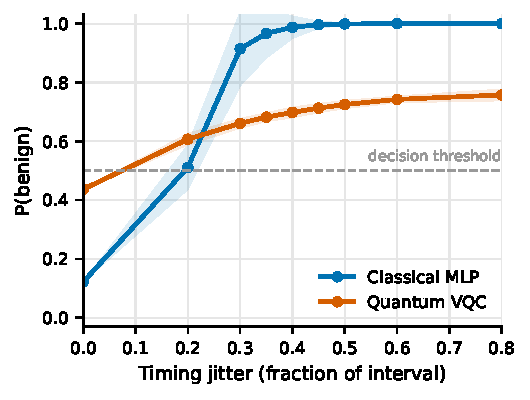
\includegraphics[width=0.7\linewidth]{fig1_evasion_curve.pdf}
\caption{Mean $P(\text{benign})$ assigned by each detector to the same swept beacon flows as timing
jitter increases (shaded band: $\pm 1$ s.d.\ across 15 instances). Both detectors cross the decision
threshold at low jitter; the VQC barely detects even a rigid beacon.}
\label{fig:evasion}
\end{figure}

\subsection{Classical vs.\ quantum: paired comparison and transferability}
\label{sec:paired}
Because the quantum and classical detectors are trained on identical inputs
(Section~\ref{sec:detectors}) and scored on the \emph{same} captured flows via the capture-once sweep
(Section~\ref{sec:paired-method}), their robustness is directly comparable.

\paragraph{No quantum robustness advantage.} Across the 15 paired beacon instances, the minimal evading
jitter was equal for the two detectors in 10 cases and lower for the VQC in 5, and \emph{never} higher
(mean difference VQC~$-$~MLP $= -0.037$). On a realistic task the quantum classifier is thus, if
anything, \emph{marginally easier} to evade, and is in no case harder. This reverses an apparent
quantum ``edge'' we observed on an earlier saturated (100\%-clean-accuracy) version of the task, which
we attribute to that task being trivially separable; once detection is realistic, the apparent
advantage disappears.

\paragraph{Transferability is asymmetric and follows detector strength.} A beacon tuned to just evade
the VQC also evaded the MLP in only 67\% of cases, whereas a beacon tuned to just evade the MLP evaded
the VQC in 100\% of cases (Table~\ref{tab:transfer}). That is, evasions crafted against the (weaker,
lower-jitter) VQC do not reliably carry to the stronger MLP, while evasions against the MLP transfer
fully to the VQC---consistent with the VQC's decision region being the more permissive of the two. An
attacker who succeeds against the stronger detector succeeds against the weaker one for free.

\begin{table}[h]
\centering
\caption{Cross-model transferability of minimal-jitter evasions ($n=15$).}
\label{tab:transfer}
\begin{tabular}{lc}
\toprule
Evasion tuned against $\rightarrow$ scored on & Transfer rate \\
\midrule
MLP $\rightarrow$ VQC & 100\% (15/15) \\
VQC $\rightarrow$ MLP & 67\% (10/15) \\
\bottomrule
\end{tabular}
\end{table}

\subsection{Adversarial-training defense and axis escalation}
\label{sec:defense}
We fold evaded beacons into training (beacon seeds 0--9) and retrain, holding out seeds 10--14 for
evaluation (Section~\ref{sec:defense-method}).

\paragraph{Hardening defeats the timing-jitter attack---at a cost.} On the held-out instances, the
jitter evasion that previously succeeded for 100\% of beacons succeeds for 0\% against both hardened
detectors. However, hardening raises the benign false-positive rate and, for the VQC, degrades clean
accuracy (Table~\ref{tab:hardened}). Teaching the detector that jittered beacons are malicious pushes it
to flag the near-identical rigid benign traffic: the VQC's benign FPR rises to 31\%. Defending the
timing axis is not free.

\begin{table}[h]
\centering
\caption{Hardened detectors: clean performance and held-out timing-jitter evasion after
adversarial training on jittered beacons.}
\label{tab:hardened}
\begin{tabular}{lccc}
\toprule
Hardened detector & Clean accuracy & Benign FPR & Held-out jitter evasion \\
\midrule
MLP (native)  & 0.825 & 0.178 & 100\% $\rightarrow$ 0\% \\
MLP (matched) & 0.857 & 0.156 & --- \\
VQC           & 0.714 & 0.311 & 100\% $\rightarrow$ 0\% \\
\bottomrule
\end{tabular}
\end{table}

\paragraph{The defense is circumvented by escalation to a second axis.} The jitter hardening can only
exploit the timing axis, so we hold timing jitter at an already-evading value and line-search the
previously-unused payload-size-jitter axis against the hardened MLP (Section~\ref{sec:defense-method}).
The hardened MLP---which the timing attack could no longer touch (0\% evasion)---is re-broken for 100\%
of beacon instances at a trivial amount of size padding (median minimal \texttt{size\_jitter} $= 0.30$,
median 4 queries to evasion; Table~\ref{tab:sizeaxis}, Fig.~\ref{fig:armsrace}). Size padding is as
functionally free as timing jitter: the beacon's control channel is unaffected.

\begin{table}[h]
\centering
\caption{Axis escalation: payload-size-jitter line search against the hardened MLP (timing jitter held
at an already-evading value), over 15 beacon instances.}
\label{tab:sizeaxis}
\begin{tabular}{lc}
\toprule
Metric & Value \\
\midrule
Evasion rate                 & 100\% (15/15) \\
Median min.\ size-jitter     & 0.30 \\
Median queries-to-evasion    & 4 \\
\bottomrule
\end{tabular}
\end{table}

\begin{figure}[h]
\centering
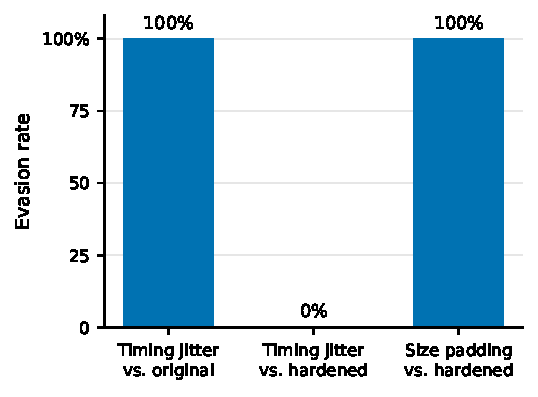
\includegraphics[width=0.7\linewidth]{fig2_arms_race.pdf}
\caption{The defense arms race against the classical MLP: the timing-jitter attack evades the original
detector (100\%), is defeated by adversarial training (0\%), and the hardened detector is re-broken by
escalation to the payload-size axis (100\%).}
\label{fig:armsrace}
\end{figure}

Single-axis adversarial training therefore does not close the vulnerability; it \emph{relocates} it to
the next functionally-free axis. Because realizable traffic offers the attacker several such axes
(timing and size here, among others), defending them one at a time is a losing exchange---the attacker
simply moves to an undefended axis at negligible cost.

% =====================================================================
\section{Discussion}
\label{sec:discussion}
\todo{Draft with co-author.} Points to develop: what the result implies for deploying flow-level C2
detectors; why the quantum model shows no robustness advantage once the task is realistic (expressivity
vs.\ the problem-space constraint); limitations (single attack family, emulated testbed, simulator-based
VQC, window-dependent features); and what a robust defense would require (the joint multi-axis space,
not single-axis hardening).

% =====================================================================
\section{Conclusion}
\label{sec:conclusion}
\todo{Draft with co-author.}

% =====================================================================
\section*{Data and code availability}
\todo{Zenodo DOI + repo URL.}

\bibliographystyle{elsarticle-num}
\bibliography{references}

\end{document}
